\section{Ziel}
In diesem Experiment soll der Faraday Effekt in GaAs gemessen werden.
\section{Theorie}
\label{sec:Theorie}
\subsection{Bandstruktur und effektive Masse}
Die Verteilung von Elektronen in Festkörpern wird üblicherweise durch die sogenannte Bandstruktur dargestellt und soll hier noch einmal kurz wiederholt werden.
Grundsätzlich unterscheidet man bei Festkörpern zwischen Metallen, Halbleitern und Isolatoren.
Jede Art von Festkörper besitzt ein Leitungsband in dem sich die Leitungselektronen befinden und Valenzbänder für die Valenzelektronen.
Die verschiedenen Festkörper unterscheiden sich in der Bandstruktur durch die verschieden großen Abstände zwischen Leitungs und Valenzbändern, siehe Abbildung \ref{fig:bandstruk}.
Bei metallen liegt die Fermi Energie in dem Leitungsband und die Bandlücke zwischen Leitungs- und Valenzband ist relativ klein, daher sind Metalle gute elektrische Leiter.
Bei Halbleitern und bei Isolatoren liegt die Fermienergie in der Bandlücke zwischen Leitungs und Valenzband. 
Isolatoren haben die größte Bandlücke und sind damit auch die schlechtesten elektrischen Leiter. 
Bei Halbleitern ist die Bandlücke relativ klein und für die Elektronen gut überwindbar.
\begin{figure}[ht]
    \centering
    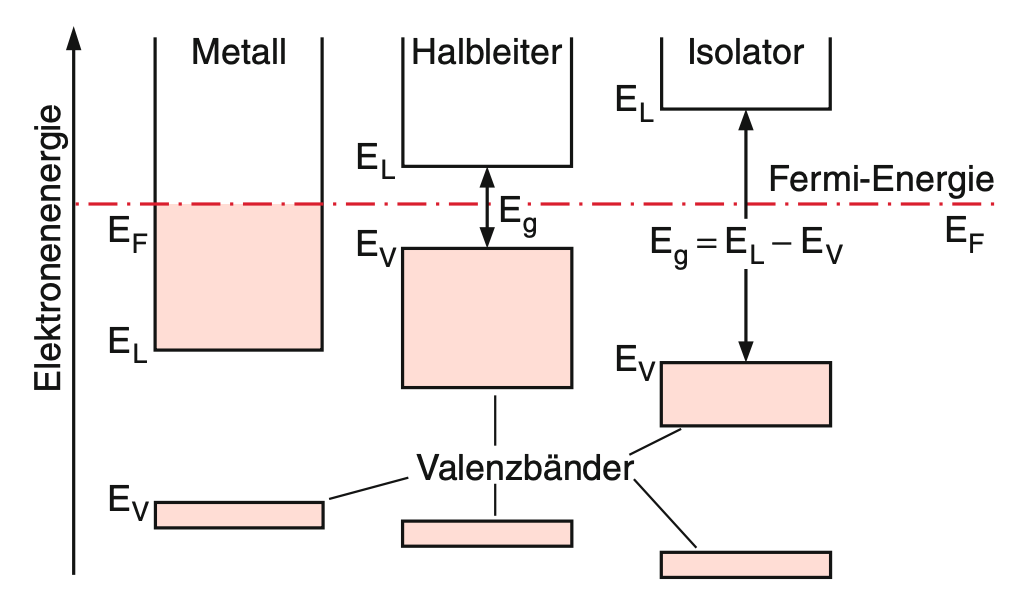
\includegraphics[scale = 0.5]{./bilder/Bandstruktur_demtroeder.png}
    \caption{Schematische Darstellung der Bandstruktur von Isolatoren und Leitern \cite{demtröder}}
    \label{fig:bandstruk}
\end{figure}

Um Elektronen im Festkörper zu beschreiben ist zu beachten, dass das Elektron nicht nur ein elektrisches Potential erfährt sondern zusätzlich noch von einem ortsabhängigem Potential beeinflusst wird.
Damit die Elektronen weiterhin als freie Elektronen beschrieben werden können modifiziert man ihre Masse zu einer effektiven Masse $m^{\*}$ die das Kristallpotential mit beachtet.

Die beschleunigung eines Elektrons in einem Festkörper lässt sich als Ableitung der Gruppengeschwindigkeit definieren:
\begin{equation}
    \vec{a} = \frac{\text{d}v_g}{\text{d}t} = \frac{1}{\hbar} \left( \frac{\text{d}^2 E}{\text{d}k^2}\right) \cdot \frac{\text{d}\vec{k}}{\text{d}t}
    \label{eqn:bewegungsgl}
\end{equation}
Wobei in Gleichung \ref{eqn:bewegungsgl} die Ableitung des Impulses nach der Zeit als Kraft geteilt durch das Plancksche Wirkungsquantum ausgedrückt werden kann.
\begin{equation}
    \vec{a} = \frac{1}{\hbar^2} \left( \frac{\text{d}^2 E}{\text{d}k^2}\right) \cdot \vec{F}
\end{equation}

Diese Formel ist kann nun als Bewegungsgleichung für die freien Elektronen betrachtet werden und die klassische Masse wird hier durch die effektive Masse ersetzt.
\begin{align}
    \vec{a} &= \frac{1}{m^{*}} \vec{F}\\
    m^{*} &= \hbar^2 \left( \frac{\text{d}^2 E}{\text{d}k^2}\right)^{-1}
\end{align}

\subsection{Dotierung von Halbleitern}
Die Dotierung von Halbleitern meint das Einfügen von Fremdatomen in das bestehende Kristallgitter um die Bandstruktur und damit auch die Leitfähigkeit des Kristalls zu verändern.
Es wird bei der Dotierung zwischen Donatoren und Akzeptoren unterschieden.
Wir betrachten hier beispielsweise einen Halbleiter mit 4-wertigen Atomen.

\subsubsection{n-Dotierung}
Als n-Dotierung bezeichnet man nun das hinzufügen von 5-wertigen Atomen in den Halbleiter.
Durch die 5-wertigkeit der neuen Atome ist jeweils eines ihrer Leitungsatome nur sehr schwach gebunden und kann als weiteres Leitungselektron fungieren.
Dieser neue Zustand für die Elektronen wird Donatorzustand genannt und befindet sich knapp unter der Fermi Energie.
Durch die nähe des Zustands zum Leitungsband, können schon kleine Energien das Elektron in das Leitungsband befördern.
\begin{figure}[ht]
    \centering
    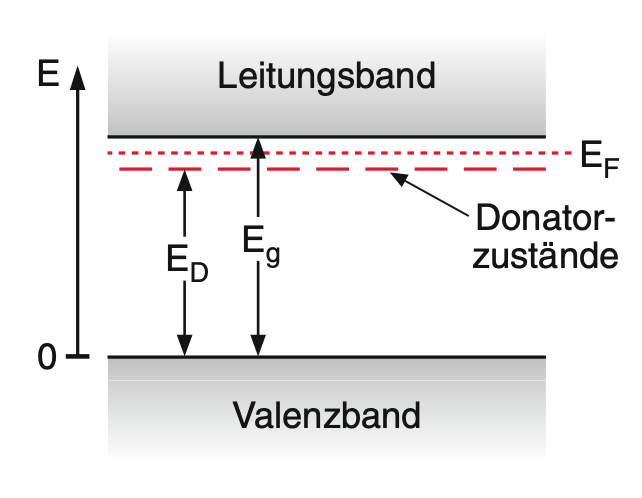
\includegraphics[scale = 0.5]{./bilder/n_Donatorschema_demtroeder.png}
    \caption{Der Donatorzustand in einem n-dotierten Halbleiter \cite{demtröder}.}
    \label{fig:n_donator}
\end{figure}

\subsubsection{p-Donatoren}

Werden dem Halbleiter niedrigwertige, zum Beispiel 3-wertige, Atome hinzugefügt, spricht man von einem p-dotierten Halbleiter. In p-dotierten Halbleitern entsteht auch ein neuer Zustand, der Akzeptorzustand, da die neuen Atome ein Atom zu wenig haben um Bindungen mit den anderen Atomen einzugehen.
Der Akzeptorzustand liegt über dem Valenzband knapp über der Fermi Energie.
Durch die nähe zum Valenzband können Elektronen schon durch geringe Energiemengen über die Fermienergie gehoben werden und sogenannte Löcher im Valenzband hinterlassen.
Die Löcher im Valenzband können als quasi-Ladungsträger die Leitfähigkeit des Halbleiters erhöhen.
\begin{figure}[ht]
    \centering
    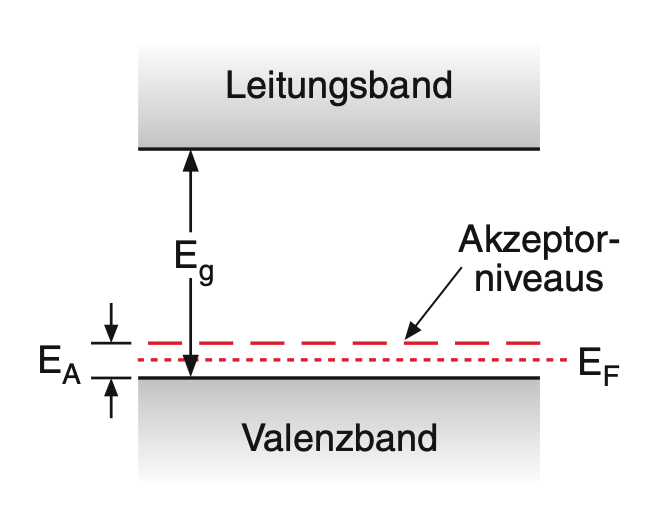
\includegraphics[scale = 0.5]{./bilder/p_Donatorschema_demtroeder.png}
    \caption{Der Akzeptorzustand in einem p-dotierten Halbleiter \cite{demtröder}.}
    \label{fig:p_donator}
\end{figure}

\subsection{Faraday Effekt}
Der Faraday Effekt beschreibt die Rotation der Polarisationsebene eines Lichtstrahls beim Durchlaufen einer !!Probe!! in einem Magnetfeld.

\subsection{Zirkulare Doppelbrechung}
Beim durchlaufen eines Mediums erzeugt Licht dort eine Polarisation proportional zur Stärke des E-Feldes der elektromagnetischen Welle.
\begin{equation}
    \vec{P} = \epsilon_0 \underline{\underline{\chi}} \vec{E}
\end{equation}
Das $\chi$ ist die Suszeptibilität und nimmt in anisotropen Kristallen im Regelfall die Form einer Matrix an.
Im Fall dieses Versuchs wird ein Suzeptibilitätstensor für doppelbrechende Materialien verwendet werden:
\begin{equation}
    \underline{\underline{\chi}} = 
    \begin{pmatrix}
        \chi_{xx} & i \chi_{xy} & 0\\
        -i \chi_{xy} & \chi_{xx} & 0\\ 
        0 & 0 & \chi_{zz}\\
    \end{pmatrix}
    \label{eqn:Suszept}
\end{equation}
Nur wenn im Suzebtibilitätstensor nicht-diagonale und konjugiert komplexe Koeffizienten auftreten kann die Doppelbrechung erklärt werden.
Mit der dielektrischen Verschiebung $\vec{D} = \epsilon_0 \vec{E} + \vec{P} $ anstelle von $\vec{E}$ eingesetzt in die Wellengleichung, liefert sich eine neue Form gemäß Formel \ref{eqn:wellengleichung}.
\begin{equation}
    \nabla \times \left( \nabla \times \vec{E} \right) = -\frac{1}{c^2} \left( 1 + \underline{\underline{\chi}} \right) \cdot \frac{\partial^2 \vec{E}}{\partial t^2}
    \label{eqn:wellengleichung}
\end{equation}
Für die z-Komponente des E-Feldes der EM-Welle ergibt sich damit
\begin{equation}
    \frac{\omega^2}{c^2} \cdot E_z = \frac{\omega^2}{c^2} \chi_{zz} \cdot E_z
\end{equation}
daher muss $E_{z}$ für den gegebenen Fall verschwinden.
Daher existiert eine nicht-triviale Lösung für $E_x$ und $E_y$ wenn die Determinante des Tensors verschwindet.
\begin{equation}
    \left( -k^2 + \frac{\omega^2}{c^2}\cdot \left( 1 + \chi_{xx} \right) \right)^2 - \left( i \cdot \frac{\omega^2}{c^2} \chi_{xy} \right)^2 = 0
\end{equation}
Diese Bedingung führt zu einschränkungen für die Wellenzahl und erzeugt zwei Lösungen für die Phasengeschwindigkeiten:
\begin{equation}
    v_{Ph_{R}} = \frac{c}{\sqrt{1+\chi_{xx} +\chi_{xy}}}  \; \; \; \;  v_{Ph_{L}} = \frac{c}{\sqrt{1+\chi_{xx} -\chi_{xy}}} 
\end{equation}
Daher bewegen sich eine linkszirkular und eine rechtszirkular laufende Welle unterschiedlich schnell durch das optische Medium.
Durch die verschiedenen Geschwindigkeiten wird innerhalb des Materials die Polarisation der Welle um den Winkel $\theta$ gedreht.
\begin{equation}
    \theta = \frac{L\omega}{2} \left( \frac{1}{v_{Ph_{R}}} - \frac{1}{v_{Ph_{L}}} \right)
\end{equation}
Die Drehung ist dabei auch von der Länge des Weges im Material und der Frequenz der EM-Welle abhängig.
Mit einer Reihenentwicklung kann der Drehwinkel abschließend durch eine Komponente der Suszeptibilität ausgedrückt werden.
\begin{equation}
    \theta \approx  \frac{L\omega}{2cn} \chi_{xy}
    \label{eqn:theta}
\end{equation}

\subsection{Faraday Effekt}
Der Faraday Effekt ist ein spezialfall der sogenannten induzierten Doppelbrechung bei Materialien die nicht doppelbrechend oder optisch aktiv sind.
Der Faraday Effekt tritt durch das anlegen eines äußeren Magnetfeldes an das isotrope Material auf.
Ein Magnetfeld $\vec{B}$ verändert dabei die Bewegungsgleichungen der Elektronen im Material.
\begin{equation}
    m \cdot \frac{\text{d}^2 \vec{r}}{\text{d}t^2} + K\cdot \vec{r} = - \text{e} \vec{E}(r)- \text{e} \frac{\text{d} \vec{r}}{\text{d}t} \times \vec{B}
\end{equation}
In dieser veränderten Bewegungsgleichung wird das angelegte Magnetfeld durch $\vec{B}$ und das elektrische Feld des Lichtes durch $\vec{E}(r)$ beschrieben.
Nun wird $\vec{r}$ und $\vec{E}(r)$ durch die bekannte Zeitabhängigkeit des elektrischen Feldes ersetzt und das Magnetfeld wird in z-Richtung angenommen.
Mit diesen änderungen ergeben sich drei Komponenten der Bewegungsgleichung.
\begin{align*}
    \left(-m\omega^2 + K\right) \cdot P_x &= N \text{e}^2\cdot E_x + i\omega P_y B\\
    \left(-m\omega^2 + K\right) \cdot P_y &= N \text{e}^2\cdot E_y - i\omega P_y B\\
    \left(-m\omega^2 + K\right) \cdot P_z &= N \text{e}^2\cdot E_z
\end{align*}
Für die Suszeptibilität wird wie zuvor besprochen der ansatz eine Doppelbrechenden Materie genutzt \ref{eqn:Suszept}
\begin{equation}
    \underline{\underline{\chi}} = 
    \begin{pmatrix}
        \chi_{xx} & i \chi_{xy} & 0\\
        -i \chi_{xy} & \chi_{xx} & 0\\ 
        0 & 0 & \chi_{zz}\\
    \end{pmatrix}
\end{equation}
Durch die Annahme dieser Suszeptibilität kann das Gleichungssystem der drei Komponenten der Polarisation gelöst werden.
Daher werden auch isotrope Medien beim Anlegen eines Magnetfeldes Doppelbrechend.
Durch einsetzen der so gewonnenen Suszeptibilität in \ref{eqn:theta} ergibt sich:
\begin{equation}
    \theta = \frac{\text{e}^3}{2c\epsilon_0 m^2} \frac{\omega^2}{\left(-\omega^2 + \frac{K}{m}\right)^2 - \left(\frac{e}{m} \cdot B\omega\right)^2} \frac{NBL}{n}
\end{equation} 

Wobei $\sqrt{\frac{K}{m}}$ einer Resonatorfrequenz für $\omega_0$ der gebundenen Ladungsträger entspricht.
$\frac{Be_0}{m}$ ist hierin eine Zyklotronfrequenz $\omega_c$, die die Umlauffrequenz der Ladungsträger mit Massde $m$ und Ladung $e_0$ angibt.
Liegt man mit der Messfrequenz unter der Resonatorfrequenz $\omega_0$ und führt anstatt der Kreisfrequenz die Wellenlänge des einfallenden Lichtes ein vereinfacht sich die Berechnung von $\theta$ zu
\begin{equation*}
    \theta(\lambda) \approx \frac{2\pi^2 \text{e}^3c}{\epsilon_0m^2\lambda^2\omega_0^4} \frac{NBL}{n}
\end{equation*}
Für freie Elektronen im Kristall wird die Gleichung noch weiter vereinfacht, allerdings muss die Masse durch die effektive Masse ersetzt werden.
Mit dieser GLeichung kann die effektive Masse durch die Messung des Faraday Winkels bestimmt werden.
\begin{equation*}
    \theta_{\text{frei}}(\lambda) \approx \frac{\text{e}^3 \lambda^2}{8 \pi^2\epsilon_0 c^3} \frac{1}{m^{*}}\frac{NBL}{n}
\end{equation*}